\chapter{Implementations}


\section{Creating AFs}
\textit{TODO: Explain AF creation algorithms (Random + Grid-Based)}



\section{BFS and DFS Approach}
\textit{TODO: BFS and DFS approach in current research + when BFS is better than DFS}

\section{Generating Semantic Sets}
\textit{TODO: Semantic sets generation algorithm}

\section{Faithful/Spurious Determination}
\textit{TODO: Determine faithful/spurious algorithm}

\section{Refuted Theories}
\textit{TODO: State refuted theories like subsets of spurious also spurious.}




REUSE THIS SOMEWHERE:

We encoded the semantics rules into Boolean formula and used the SAT-Solver to evaluate them. To cover all possibilities of AFs, we generalized the formulas and used short notation to concatinate the variables. Let us have a look at a concrete example with an abstract clustered AF $\mathtt{\hat{G}=(\hat{A}, \hat{R})}$ defined in \cref{af:backgroundSATExample1}.



\begin{figure}[h]
    \centering
    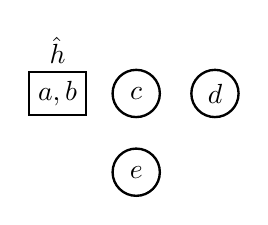
\begin{tikzpicture}
        % Singletons
        \def \cx{1}     \def \cy{0}
        \def \dx{2}     \def \dy{0}
        \def \ex{1}     \def \ey{-1}
        \def \hx{0}     \def \hy{0}

        \node[rectangle, draw, line width=0.3mm] at (\hx, \hy) {$a,b$};
        \node at (0, 0.55) {$\hat{h}$};
        \draw[line width=0.3mm] (\cx, \cy) circle (0.3) node[anchor=center]{$c$};
        \draw[line width=0.3mm] (\dx, \dy) circle (0.3) node[anchor=center]{$d$};
        \draw[line width=0.3mm] (\ex, \ey) circle (0.3) node[anchor=center]{$e$};

        % Attacks
        \DrawAttackHorizontal{R}{\hx+0.1}{\hy}{\cx}{\cy}
        \DrawSelfAttackRightSingleton{\cx}{\cy}
        \DrawAttackHorizontal{R}{\cx}{\cy}{\dx}{\dy}
        \DrawAttackVertical{D}{\cx}{\cy}{\ex}{\ey}
        \DrawAttackDiagonal{PB}{\dx}{\dy}{\ex}{\ey}
    \end{tikzpicture}
    \caption{Abstract AF $\mathtt{\hat{G}}$}
    \label{af:backgroundSATExample1}
\end{figure}


\paragraph{For-OR} To concatinate all the singletons of the AF $\hat{G}$, we can use the following notation:

$$
\bigvee_{a \in \hat{G}_{\!S\!I\!N\!G\!L\!E}} a = c \lor d \lor e
$$

\paragraph{For-AND} To concatinate all the singletons of the AF $\hat{G}$, we can use the following notation:

$$
\bigwedge_{a \in \hat{G}_{\!S\!I\!N\!G\!L\!E}} a = c \land d \land e
$$

\paragraph{For-Attacks} To iterate over the attacks $\hat{R}$ we can extract it from the AF as tuple and address the attacker $a$ and defender $b$:

$$
\bigwedge_{(a, b) \in \hat{R}, a\in \hat{G}_{\!S\!I\!N\!G\!L\!E}} \big( a \lor b \big) = (c \lor c) \land
(c \lor d) \land (c \lor e) \land (e \lor d) \land (d \lor e)
$$